\section{Cronograma}
Para el proyecto, se ha establecido un cronograma de actividades que será llevado a cabo por un solo estudiante.
Es importante destacar que todas las actividades mencionadas se llevarán a cabo en el orden en que se presentan en el cronograma y se ajustarán según el tiempo disponible y la complejidad de cada tarea. 
\begin{table}[h!]
\centering
\begin{tabular}{|p{1cm}|p{4cm}|p{5cm}|p{5cm}|}
\hline
No actividad & Nombre de tarea & Objetivo & Resultados esperados \\
\hline
1 & Análisis y requerimientos del sistema &  Determinar y explicar los procesos que se llevarán a cabo dentro del sistema y el comportamiento de los actores. Enumerar los requisitos que debe cumplir el sistema para un buen funcionamiento. & Diagramados que describan
los procesos del sistema y el
comportamiento de los actores
(Casos de uso, secuencia,
entre otros), ocupando
diagramado UML. Listado con
los elementos que requiere el
sistema, así como los aspectos
que debe cumplir. \\
\hline
2 & Recopilación de datos de precursores sísmicos & Recopilar información relevante & Obtener datos para seleccionar base de datos \\
\hline
3 & Diseño del esquema de base de datos & Diseñar una estructura adecuada para almacenar los datos recopilados & Esquema de base de datos diseñado y tablas o colecciones creadas \\
\hline
4 & Selección de servidor & Análisis y elección de servidor, contratación de un servicio en la nube o montar un servidor local &  Tener un sistema de servidor adecuado y eficiente que satisfaga las necesidades\\
\hline
5 & Aplicación de métodos estadísticos avanzados & Analizar patrones de sismicidad y correlaciones temporales & Resultados del análisis estadístico de los datos \\
\hline
6 & Análisis de precursores sísmicos específicos & Utilizar modelos matemáticos y algoritmos para analizar precursores sísmicos & Resultados del análisis de precursores sísmicos \\
\hline
7 & Identificación de requisitos de visualización & Determinar qué tipos de gráficos, tablas o mapas son necesarios & Requisitos de visualización identificados \\
\hline
8 & Elección de biblioteca o herramienta de visualización & Seleccionar una herramienta para crear visualizaciones basadas en web & Herramienta de visualización seleccionada \\
\hline
9 & Integración del sistema & Unir todos los componentes en un sistema unificado & Sistema integrado y funcional \\
\hline
\end{tabular}

\caption{Cronograma de actividades}
\end{table}

 \begin{figure}[H]
    \centering
    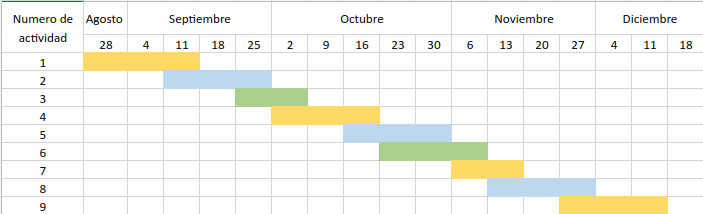
\includegraphics[width=1\textwidth]{img/crono.png}
    \caption{Cronograma de actividades}
    \label{fig:Cronograma de actividades}
\end{figure}